\documentclass[a4paper,12px]{article}
\usepackage{graphicx}
\usepackage[english]{babel}
\usepackage{fullpage}
\usepackage{xfrac}
\usepackage{fancyhdr}
\usepackage{lastpage}
\usepackage{xifthen}
\usepackage[linesnumberedhidden, titlenotnumbered]{algorithm2e}
\usepackage{lipsum}
\usepackage{hyperref}
\usepackage{array}
\usepackage{tabularx}
\usepackage{caption}
\usepackage{amsfonts}
\usepackage{amssymb}
\usepackage{amsmath}
\usepackage{mathtools}
\usepackage{placeins}
\usepackage{enumitem}
\usepackage[noabbrev]{cleveref}
\usepackage[utf8]{inputenc}
\usepackage{multirow}

\usepackage{minted}
\usepackage{listings}
\usepackage{dsfont}
\usepackage{units}

\pagestyle{fancy}
\lhead{
\includegraphics[width=7cm]{logoUvA}}
\rhead{\footnotesize \textsc {Report\\ \opdracht}}
\lfoot%
{%
    \footnotesize \studentA%
    \ifthenelse{\isundefined{\studentB}}{}{\\ \studentB}
    \ifthenelse{\isundefined{\studentC}}{}{\\ \studentC}
    \ifthenelse{\isundefined{\studentD}}{}{\\ \studentD}
    \ifthenelse{\isundefined{\studentE}}{}{\\ \studentE}
}
\cfoot{}
\rfoot{\small \textsc {Page \thepage\ of~\pageref{LastPage}}}
\renewcommand{\footrulewidth}{0.5pt}

\fancypagestyle{firststyle}
{%
    \fancyhf{}
    \renewcommand{\headrulewidth}{0pt}
    \chead{
\includegraphics[width=7cm]{logoUvA}}
    \rfoot{\small \textsc {Page \thepage\ of~\pageref{LastPage}}}
}

\setlength{\topmargin}{-0.3in}
\setlength{\textheight}{630pt}
\setlength{\headsep}{40pt}
\setlength{\parindent}{0pt}

% =================================== DOC INFO ===================================

\newcommand{\opdracht}{Theoretical Excercises}
\newcommand{\titel}{Labs week 2}
\newcommand{\docent}{Alban Ponse, Bob Diertens}
\newcommand{\cursus}{Theoretische aspecten van de Programmatuur}
\newcommand{\vakcode}{}
\newcommand{\datum}{\today}
\newcommand{\studentA}{Maico Timmerman}
\newcommand{\uvanetidA}{10542590}
%\newcommand{\studentB}{Tim van Zalingen}
\newcommand{\uvanetidB}{10784012}
% \newcommand{\studentC}{Boudewijn Braams}
\newcommand{\uvanetidC}{10401040}
% \newcommand{\studentD}{Govert Verkes}
\newcommand{\uvanetidD}{10211748}
%\newcommand{\studentE}{Naam student 5}
\newcommand{\uvanetidE}{UvAnetID student 5}

% ===================================  ===================================

\begin{document}
\thispagestyle{firststyle}
\begin{center}
    \textsc{\Large \opdracht}\\[0.2cm]
    \rule{\linewidth}{0.5pt} \\[0.4cm]
    {\huge \bfseries \titel}
    \rule{\linewidth}{0.5pt} \\[0.2cm]
    {\large \datum\\[0.4cm]}

    \begin{minipage}{0.4\textwidth}
        \begin{flushleft}

            \emph{Student:}\\
            {\studentA\\ {\small \uvanetidA\\[0.2cm]}}
            \ifthenelse{\isundefined{\studentB}}{}{\studentB\\ {\small \uvanetidB\\[0.2cm]}}
        \end{flushleft}
    \end{minipage}~%
    \begin{minipage}{0.4\textwidth}
        \begin{flushright}
            \emph{Lecturers:} \\
            \docent\\[0.2cm]
            \emph{Course:} \\
            \cursus\\[0.2cm]
            % \emph{Student:}\\
            \ifthenelse{\isundefined{\studentC}}{}{\studentC\\ {\small \uvanetidC\\[0.2cm]}}
            \ifthenelse{\isundefined{\studentD}}{}{\studentD\\ {\small \uvanetidD\\[0.2cm]}}
            \ifthenelse{\isundefined{\studentE}}{}{\studentE\\ {\small \uvanetidE\\ [0.2cm]}}
        \end{flushright}
    \end{minipage}\\[1 cm]
\end{center}


% =================================== CONTENTS ===================================

% \tableofcontents

\newcommand{\Sum}[2]{\sum^{#2}_{#1}}
\newcommand{\E}[1]{{\mathbb{E}\left[#1\right]}}
\newcommand{\var}[1]{{\text{var}\left[#1\right]}}
\newcommand{\diffpart}[1]{\frac{\partial}{\partial{} #1}}
\newcommand{\?}{\stackrel{?}{=}}
\newcommand{\intinf}{\int\limits_{-\infty}^{\infty}}
\newcommand{\intnulinf}{\int\limits_{0}^{\infty}}
\newcommand{\intpi}{\int\limits_{0}^{2\pi}}
\newcommand{\argmin}[1]{\underset{#1}{\mathop{\mathrm{argmin}}}}
\newcommand{\argmax}[1]{\underset{#1}{\mathop{\mathrm{argmax}}}}
\definecolor{bg}{rgb}{0.95,0.95,0.95}
% =================================== MAIN TEXT ===================================


\section{MSPea (eval \& apply)}
\subsection{$k = k1\cdot k2+k3\cdot k4$}
Multiplication in MSPea is done by setting the return value $y$ to 0 and then adding $x1$ to $y$, $x2$ times. If $x1$ is $0$, then no increments are made and if $x2$ is 0, then 0's will be added, thus reassuring the behaviour of multiplication with 0.

\inputminted[bgcolor=bg]{C}{mult.mspea}

\begin{figure}[h]
    \centering
    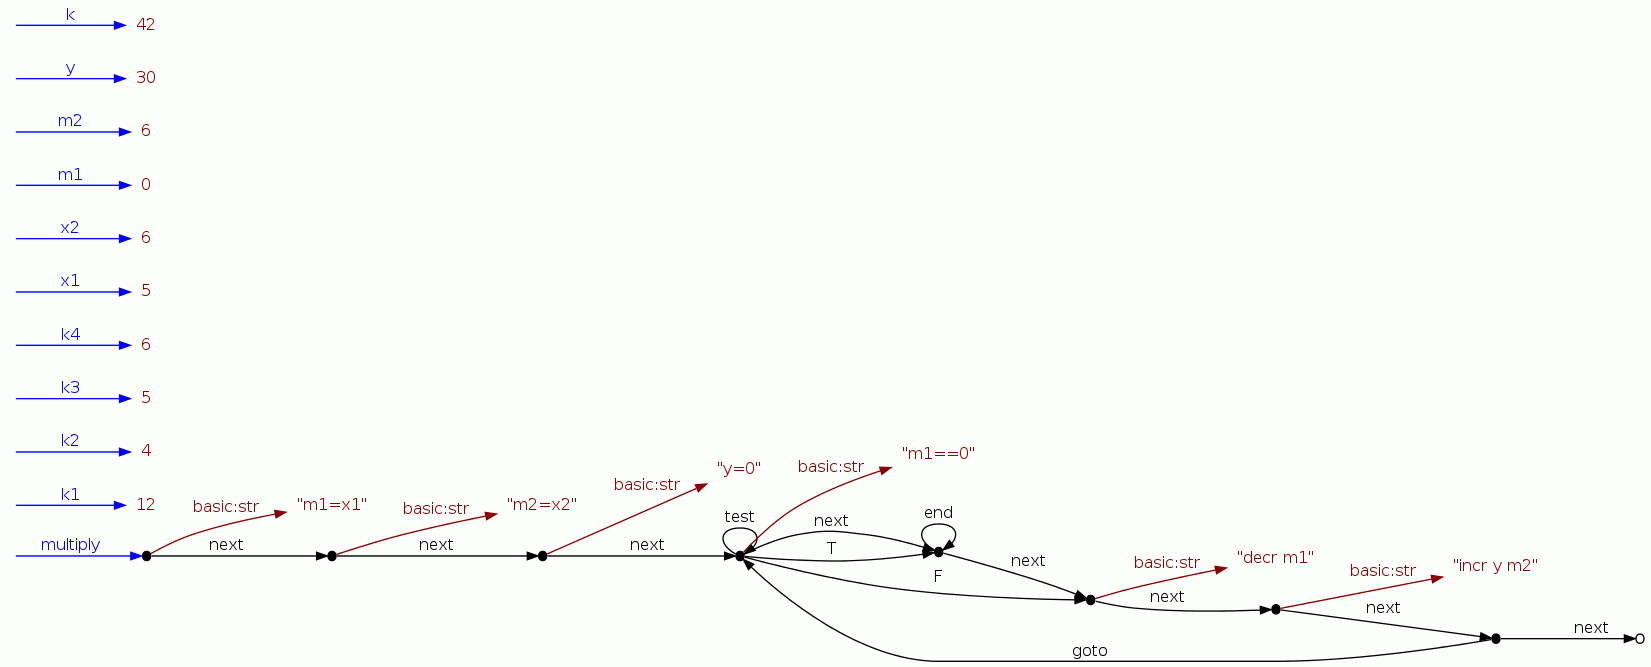
\includegraphics[width=0.8\linewidth]{mult_mspea.png}
    \caption{State after calculating $k = 3\cdot4 + 5\cdot6$}
\end{figure}
\FloatBarrier%

\subsection{$k = k1^{k2}+k3^{k4}$}
Power is implemented as a series of multiplications with a (sub) result stored in $y$. The multiplication subroutine is reused. Just like with multiplication the edge case of taking $x^0$ is assured, by setting the default value of $y$ to 1, after which there will be $x2$-times multiplications of the (sub) result with $x1$.

\inputminted[bgcolor=bg]{C}{power.mspea}

\begin{figure}[h]
    \centering
    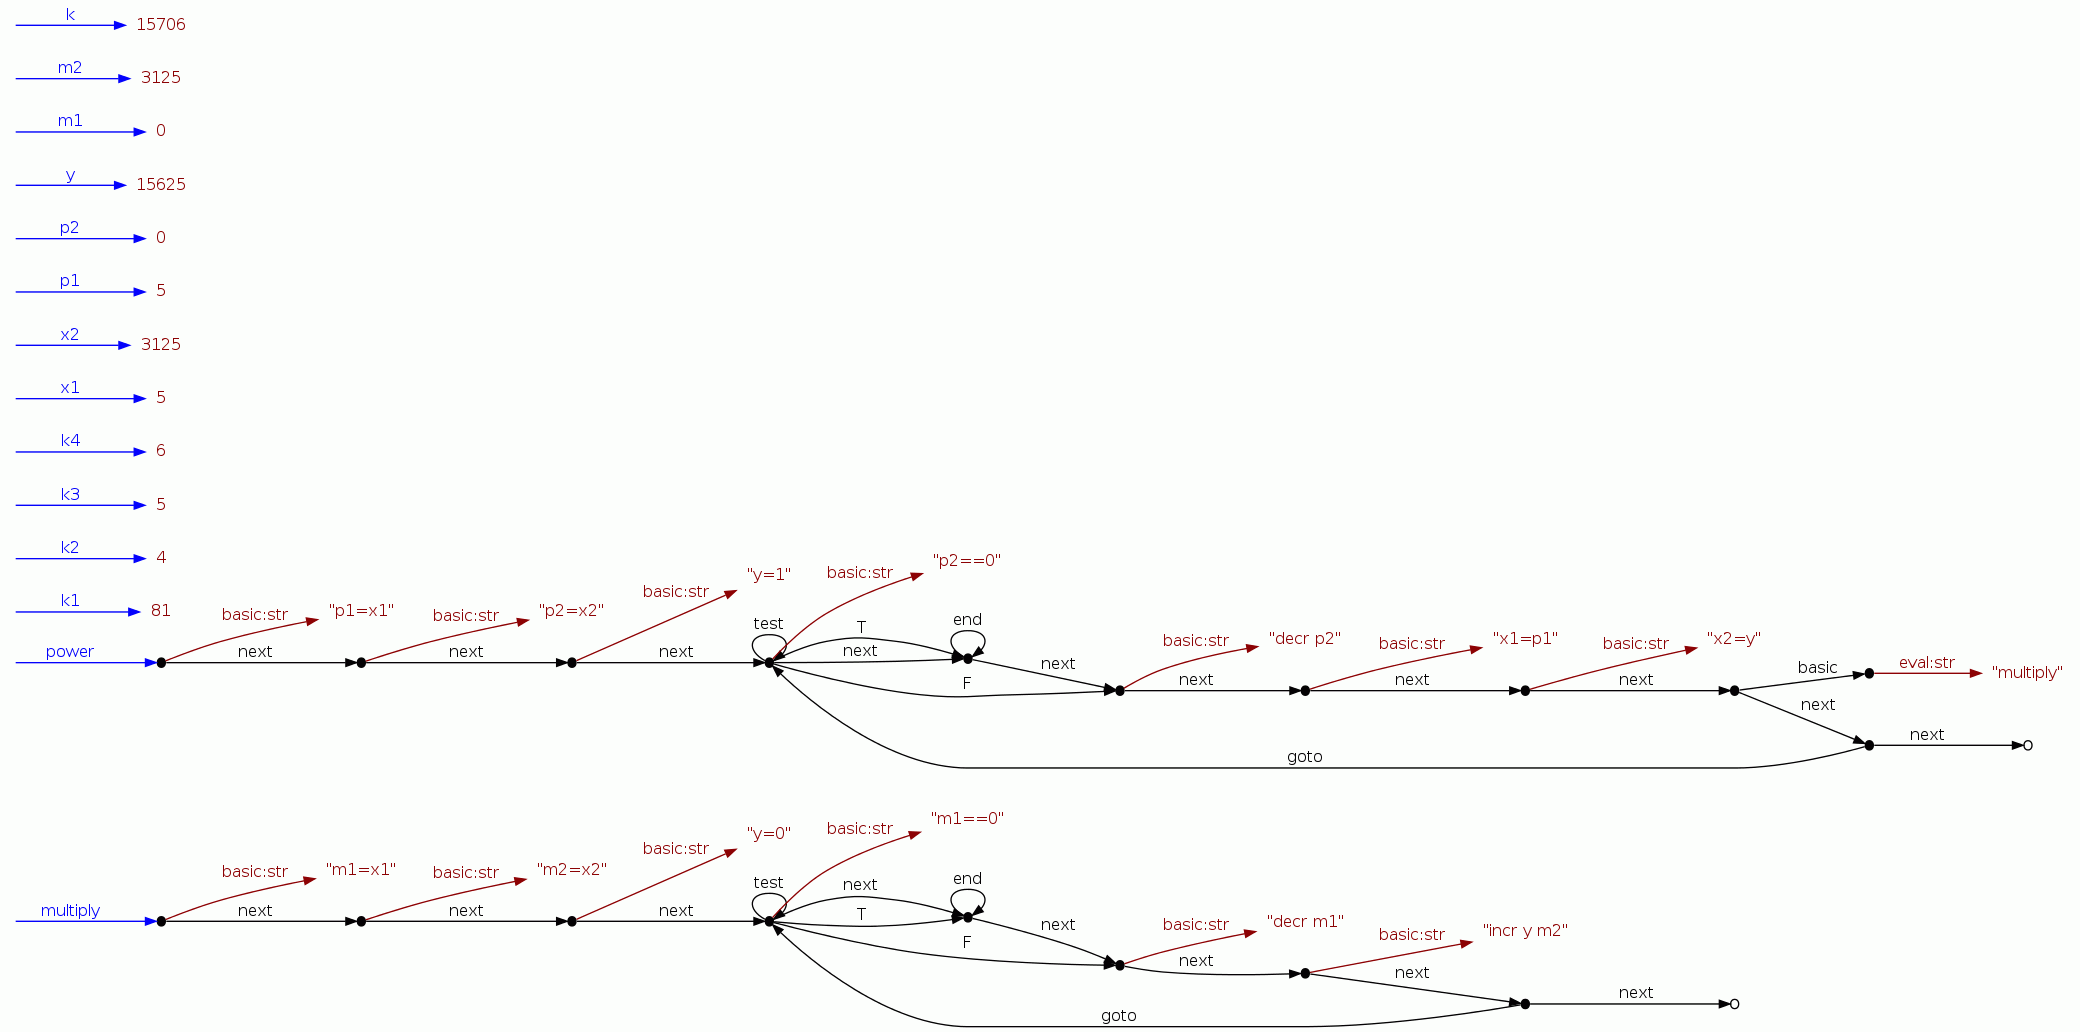
\includegraphics[width=0.8\linewidth]{power_mspea.png}
    \caption{State after calculating $k = 3^4 + 5^6$}
\end{figure}
\FloatBarrier%

\subsection{Reversing words}
Due to name collision, globals cannot be used when dealing with recursive functions. For that reason a stack is created. $S$ being the bottom of the stack and $SP$ the focus for the current state of the stack. Two subroutines are introduced. One to push a new state to the stack and one for popping the last state of the stack and cleaning the variables. Every state has a variable $v$ to store information about that state.

Reversing the string is done by taking the first character of the string saving it on the stack. After that, the algorithm will recurse to reverse the rest of the word. When the original string is empty, the function will then append the stack-saved variables to the end of the string by popping all the states.

\inputminted[bgcolor=bg]{C}{reverse.mspea}

\begin{figure}[h]
    \centering
    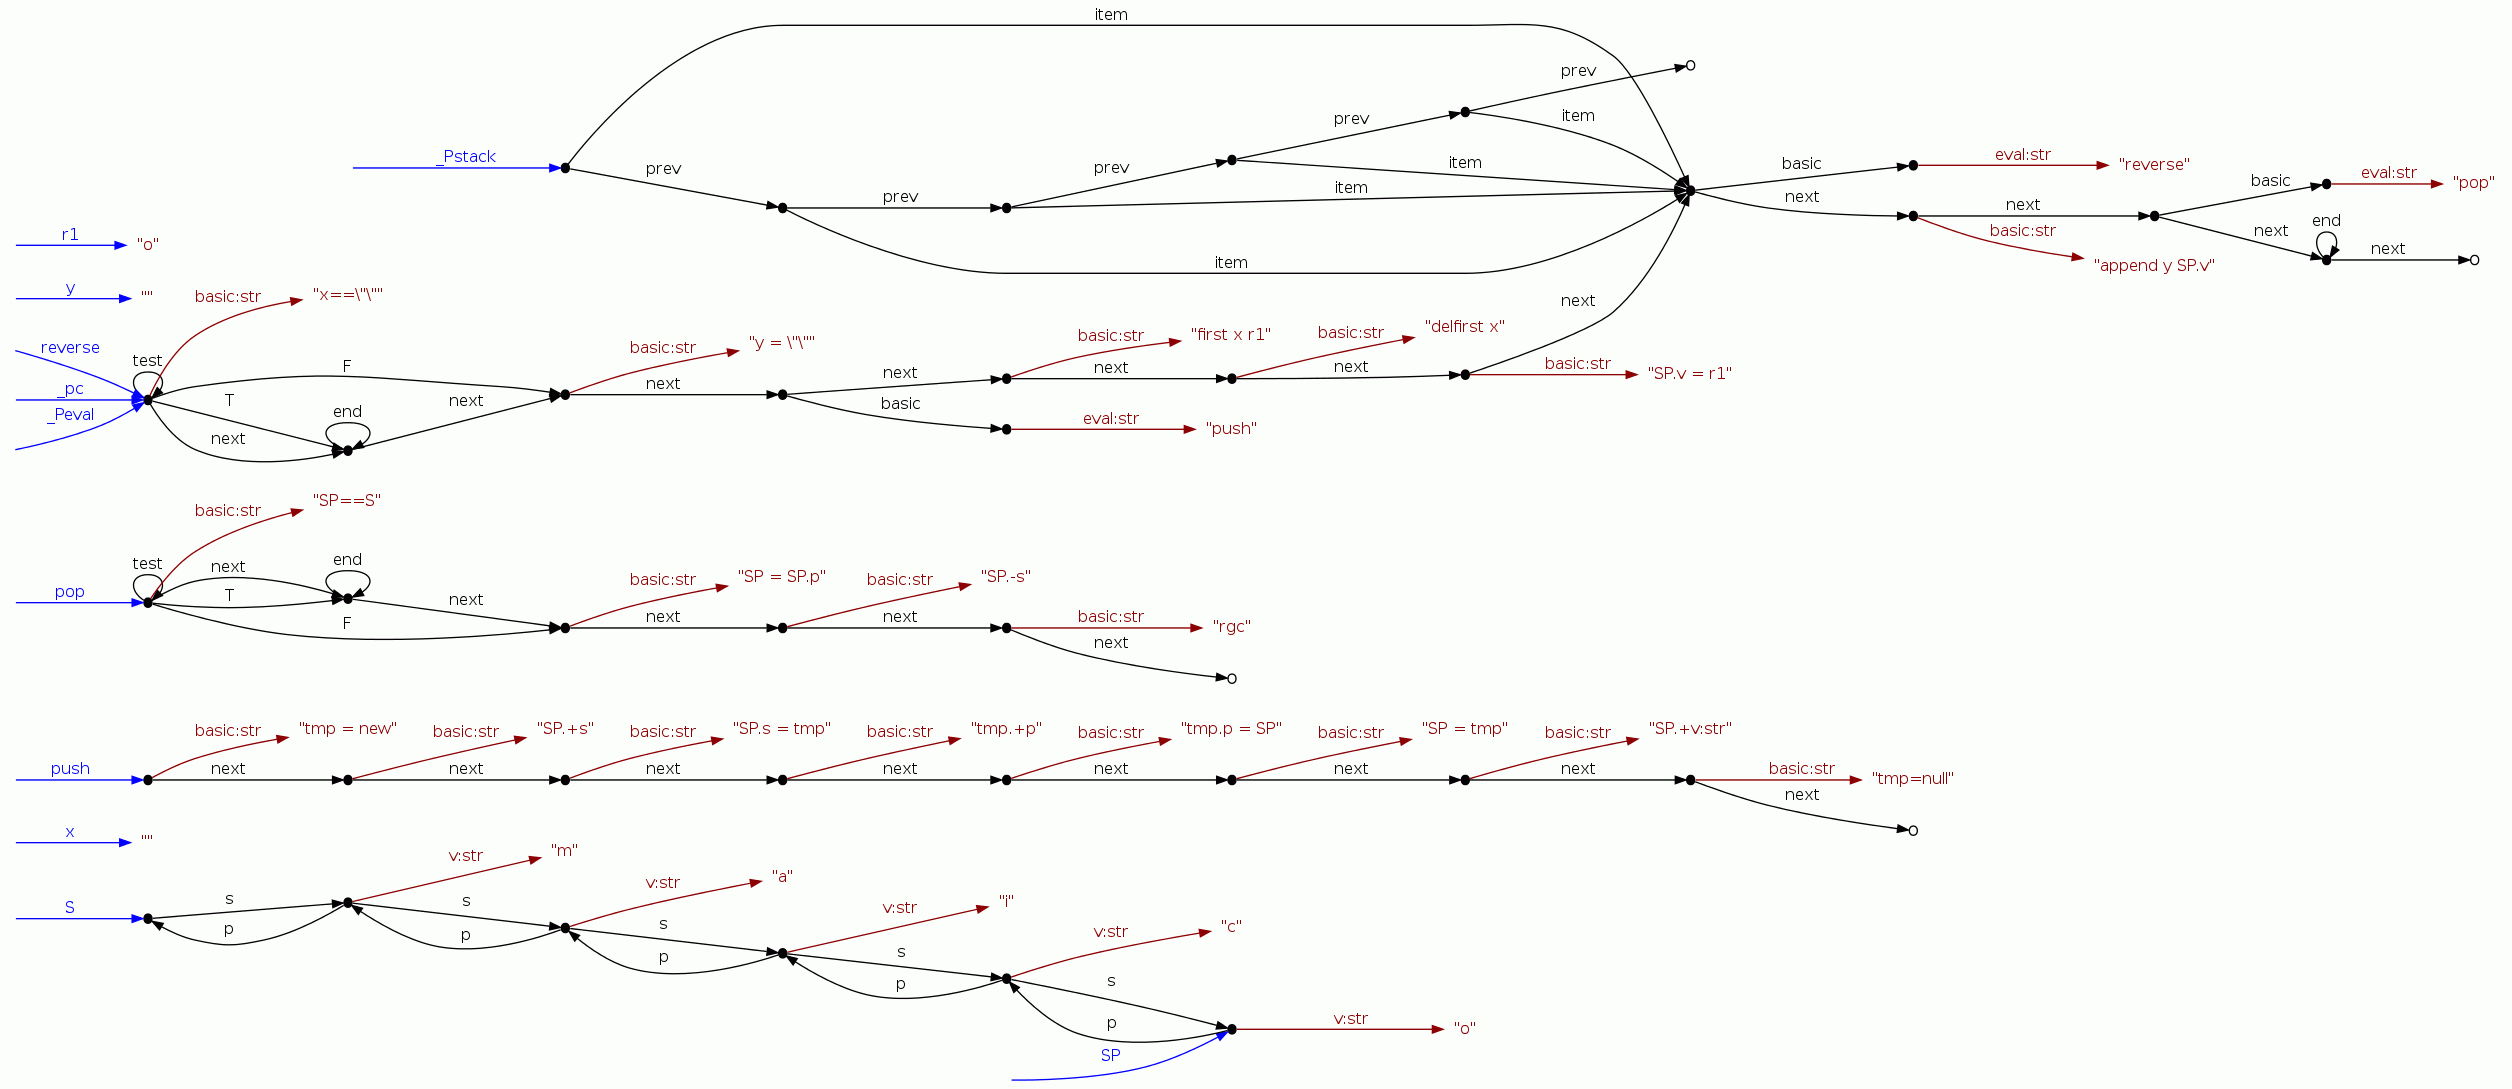
\includegraphics[width=0.8\linewidth]{reverse2_mspea.png}
    \caption{State while calculating the reverse of ``maico''.}
\end{figure}
\FloatBarrier%
\begin{figure}[h]
    \centering
    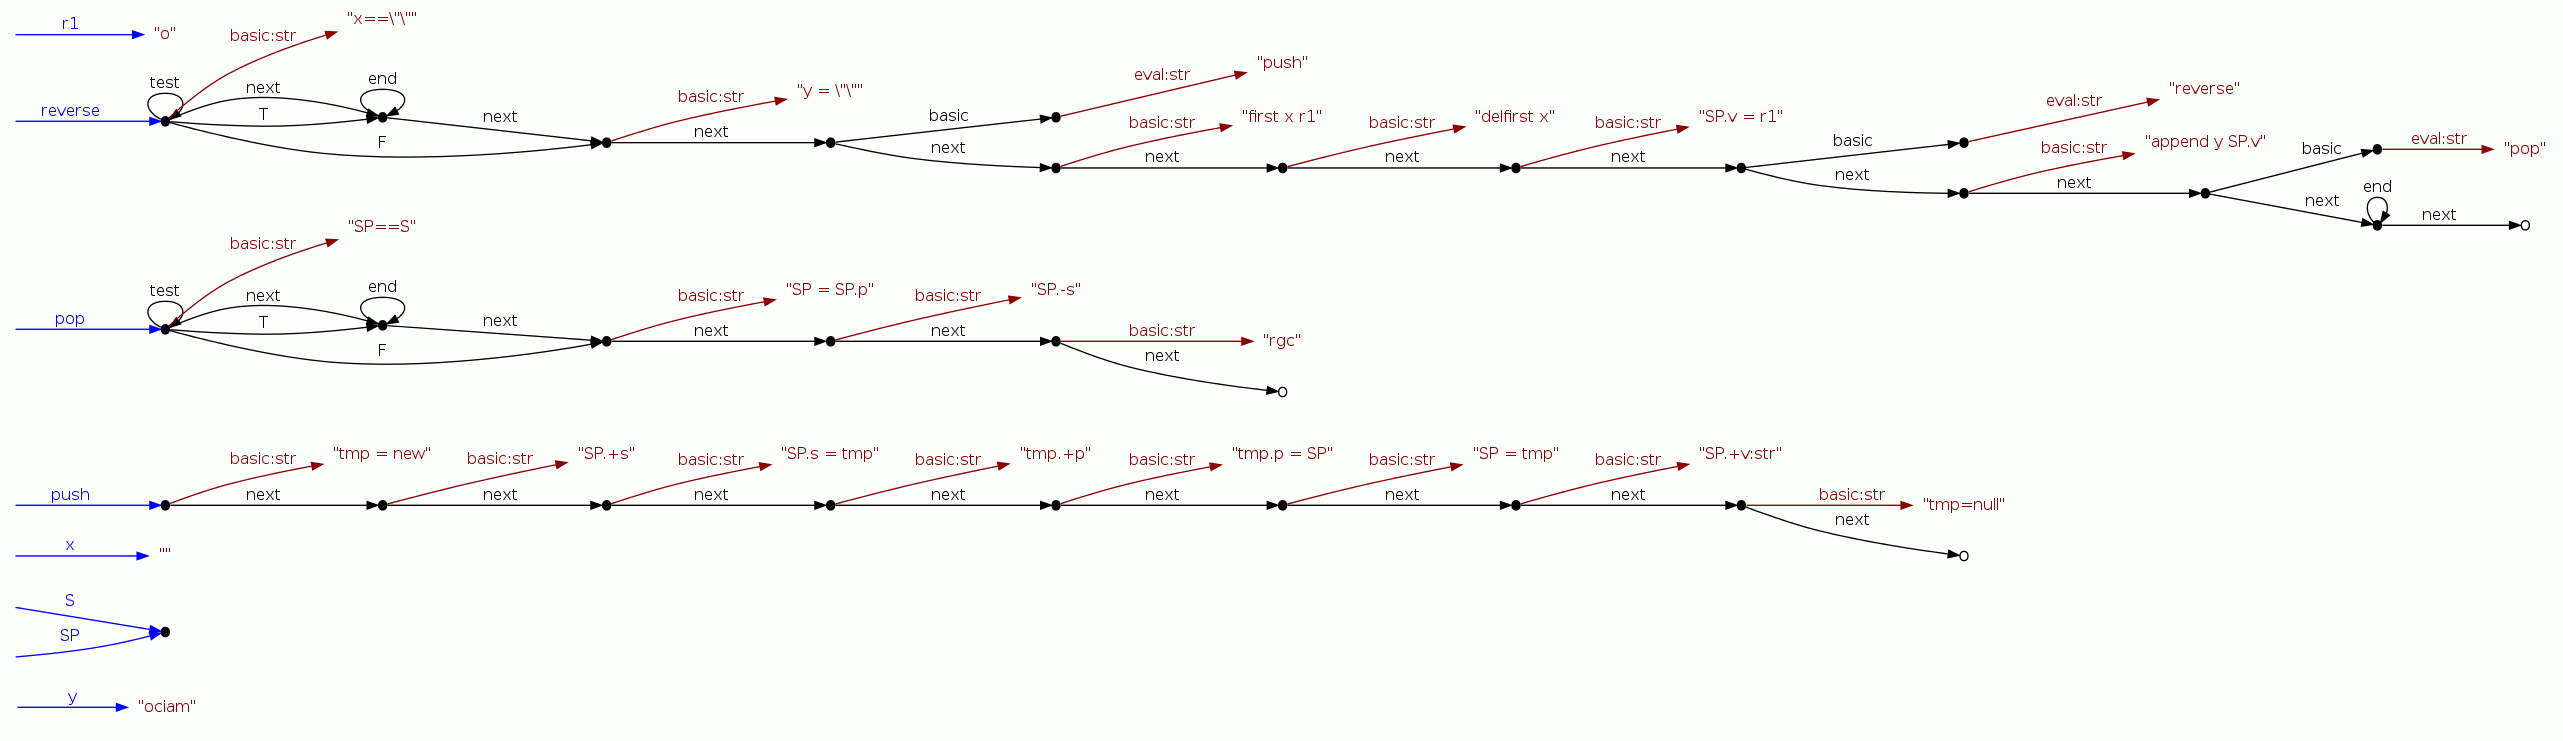
\includegraphics[width=0.8\linewidth]{reverse_mspea.png}
    \caption{State after calculating the reverse of ``maico''.}
\end{figure}
\FloatBarrier%



\section{MSPfunc (functions)}
\subsection{$k = k1\cdot k2+k3\cdot k4$}
The algorithm for multiplication in MSPfunc is exactly the same as the subroutine used in MSPea, however all variables are converted to local variables ($<>$).

\inputminted[bgcolor=bg]{C}{mult.mspfunc}

\begin{figure}[h]
    \centering
    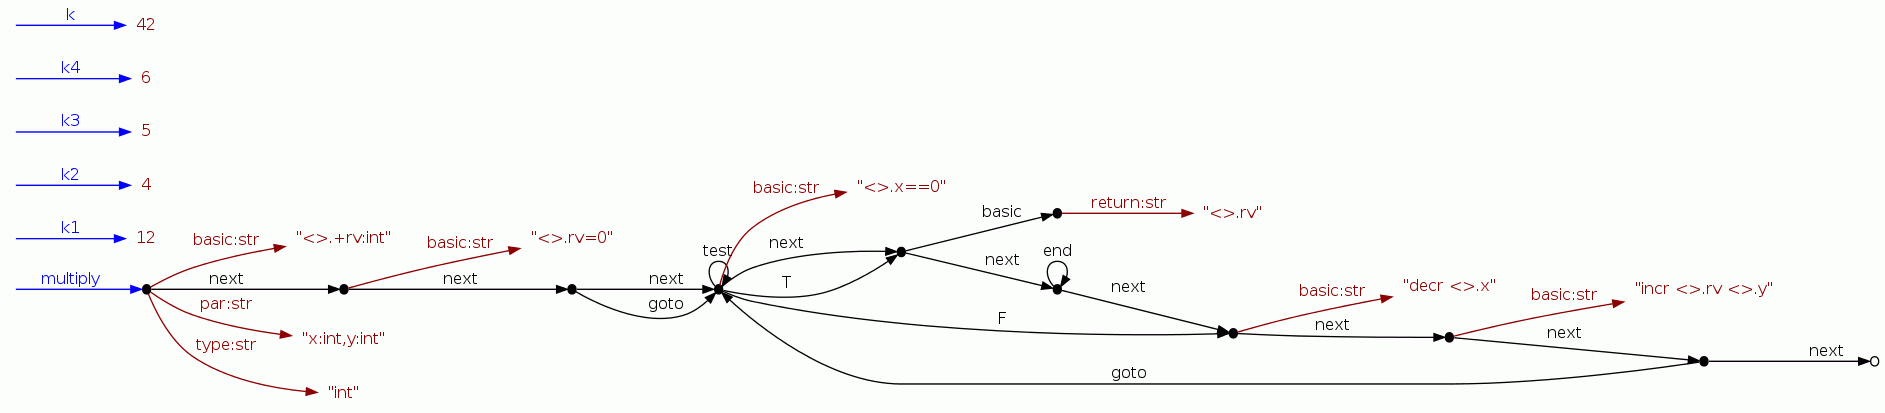
\includegraphics[width=\linewidth]{mult_mspfunc.png}
    \caption{State after calculating $k = 3\cdot4 + 5\cdot6$}
\end{figure}
\FloatBarrier%

\subsection{$k = k1^{k2}+k3^{k4}$}
The algorithm for power in MSPfunc is exactly the same as the subroutine used in MSPea, however all variables are converted to local variables ($<>$).

\inputminted[bgcolor=bg]{C}{power.mspfunc}

\begin{figure}[h]
    \centering
    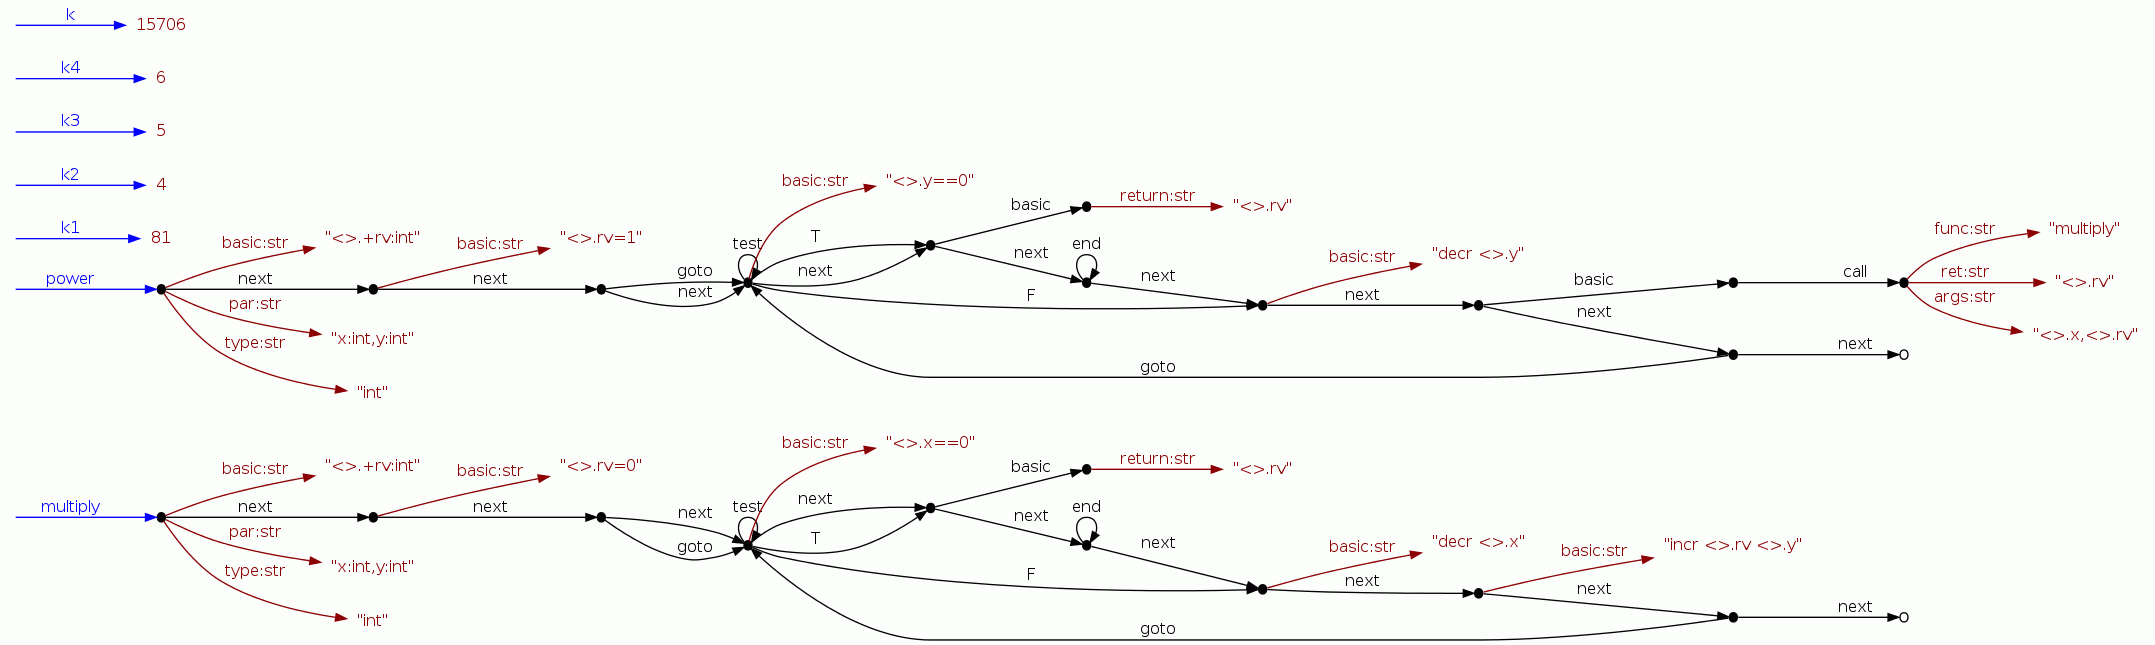
\includegraphics[width=\linewidth]{power_mspfunc.png}
    \caption{State after calculating $k = 3^4 + 5^6$}
\end{figure}
\FloatBarrier%

\subsection{revesing words}
Reversing words using MSPfunc is easier then reversing in MSPea, as the stack based variables are already implemented. By appending the first character of the string to the end of reversed string, an recursive algorithm is created.

\inputminted[bgcolor=bg]{C}{reverse.mspfunc}


\begin{figure}[h]
    \centering
    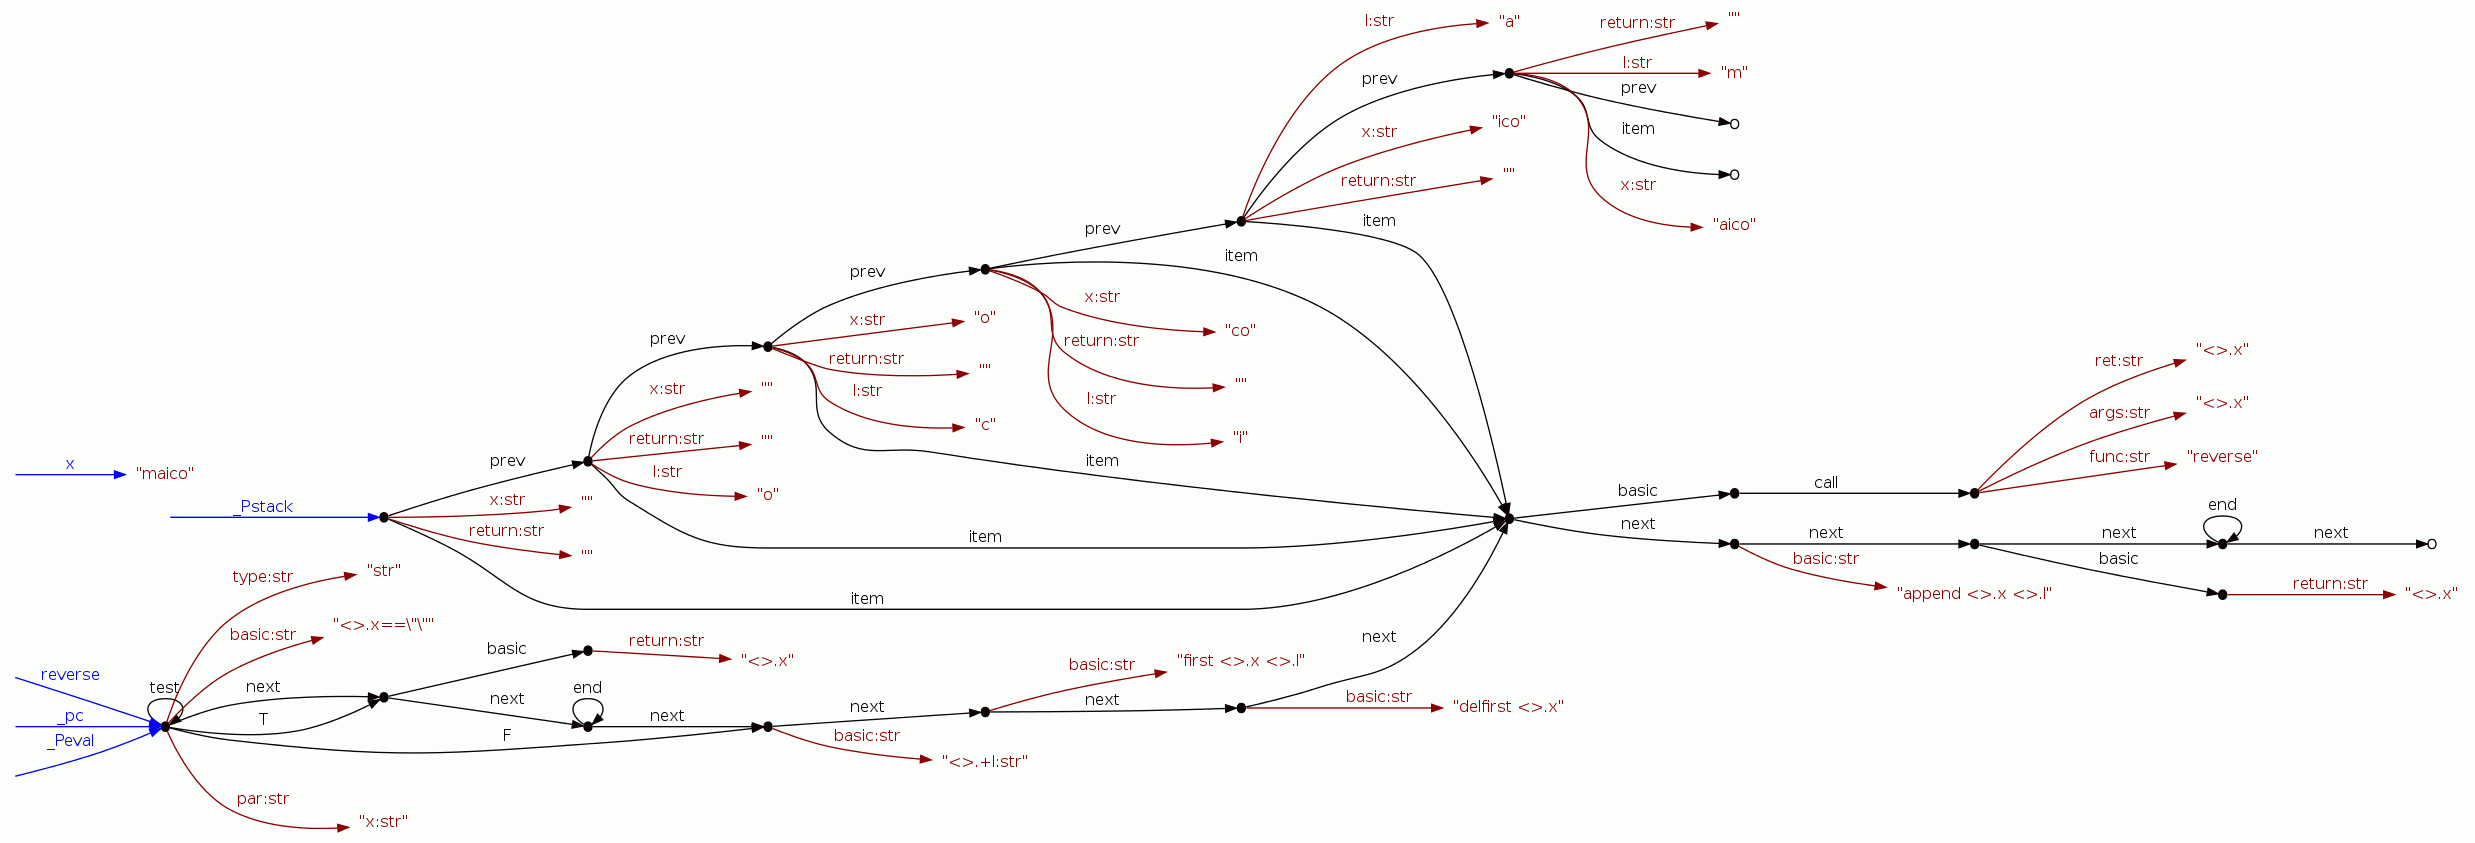
\includegraphics[width=0.8\linewidth]{reverse2_mspfunc.png}
    \caption{State while calculating the reverse of ``maico''.}
\end{figure}
\FloatBarrier%
\begin{figure}[h]
    \centering
    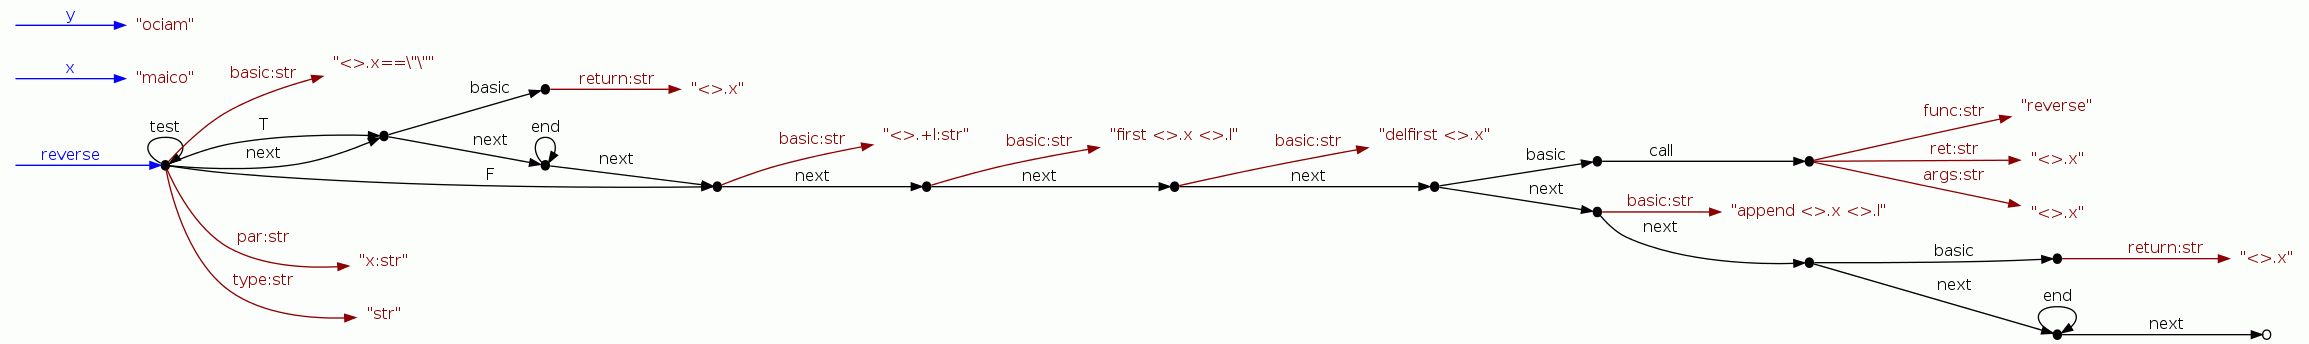
\includegraphics[width=0.8\linewidth]{reverse_mspfunc.png}
    \caption{State after calculating the reverse of ``maico''.}
\end{figure}
\FloatBarrier%


% =================================== REFERENCES ===================================

% \clearpage

% \bibliographystyle{apalike}
% \bibliography{report}

\end{document}
